% 使用 extarticle 以支援範本要求的 9-point 基礎字體 [cite: 21, 22]
\documentclass[twocolumn, 9pt]{extarticle}

\usepackage[utf8]{inputenc}
% --- 加入這段來支援中文 ---
% 如果您是在自己的 Windows 電腦上跑，可以加上下面這行來指定字體 (Overleaf 用戶建議先標註掉)
% \setCJKmainfont{微軟正黑體} 
% -------------------------

% ---- 頁面大小與邊界設定 ----
% 頂部: 1.9cm, 底部: 2.54cm, 左右: 1.9cm [cite: 17, 18]
\usepackage[top=1.9cm, bottom=2.54cm, left=1.9cm, right=1.9cm]{geometry}

% 欄間距 (Gutter) 設定為 0.83 cm [cite: 18]
\setlength{\columnsep}{0.83cm}

% ---- 字體設定 ----
% 內文使用 Times Roman (mathptmx) [cite: 21]
\usepackage[T1]{fontenc}    % 必須加入，否則粗斜體會失效
\usepackage{newtxtext} % 比 mathptmx 更穩定支援 9pt 的粗斜體


% 標題與作者資訊使用 Helvetica (helvet) [cite: 27]
\usepackage[scaled]{helvet} 
\usepackage{authblk}
\usepackage{setspace}
\usepackage{graphicx} 
\graphicspath{{./figures/}}
\usepackage{subcaption}
\usepackage{amsmath}
\usepackage{booktabs}
\usepackage{multirow}
\usepackage{hyperref}
\usepackage{enumitem}
\usepackage{placeins}
\usepackage{tabularx}
\usepackage{float}       % 提供 [H] 強制定位
\usepackage{placeins}    % 提供 \FloatBarrier
\usepackage{enumitem}    % 提供 nosep 縮減列表間距
\usepackage{balance}
\usepackage{flafter}
\setcounter{secnumdepth}{4}

% ---- 章節標題格式設定 (titlesec) ----
\usepackage{titlesec}

% 1. 主章節: Times New Roman 12-point 粗體、全大寫、靠左，上方 6-point 空白
% 【修正】加上 \selectfont，並將 \MakeUppercase 移至最後的括號
\titleformat{\section}{\rmfamily\fontsize{12}{14}\selectfont\bfseries\uppercase}{\thesection.}{1em}{}
\titlespacing*{\section}{0pt}{6pt}{*0}

% 2. 子章節: Times New Roman 12-point 粗體
% 【修正】加上 \selectfont
\titleformat{\subsection}{\rmfamily\fontsize{12}{14}\selectfont\bfseries}{\thesubsection}{1em}{}

% 3. 次子章節: Times New Roman 11-point 斜體，上方 6-point 空白
% 【修正】加上 \selectfont
\titleformat{\subsubsection}{\rmfamily\fontsize{11}{13}\selectfont\itshape}{\thesubsubsection}{1em}{}

% 4. 次次子章節 (5.1.1.1 等級): Times New Roman 11-point 斜體
% 【修正】加上 \selectfont
\titleformat{\paragraph}{\rmfamily\fontsize{11}{13}\selectfont\itshape}{\theparagraph}{1em}{}
\titleformat{\subsubsubsection}{\rmfamily\fontsize{11}{13}\selectfont\itshape}{\theparagraph}{1em}{}

% ---- 圖表說明文字格式 ----
% 說明文字使用 9-point 粗體 [cite: 57]
\usepackage[font=bf, labelsep=period]{caption}

% ---- 頁首、頁尾與頁碼 ----
% 提交時不得包含頁首、頁尾或頁碼 
\pagestyle{empty} 

% ---- 參考文獻 ----
% 範本要求使用 ACM Reference format (編號列表) [cite: 44]
\usepackage[
  style=numeric, % 改為標準數字編號格式
  sorting=none
]{biblatex}
\addbibresource{sample.bib}
\urlstyle{same} % 1. 讓所有網址與 DOI 連結的字體，跟隨內文目前的字體（不再是打字機字體）
\DeclareFieldFormat{doi}{doi: \href{https://doi.org/#1}{#1}} % 2. 強制把大寫 DOI 改成小寫 doi，並保持超連結功能

%%%%%% Title %%%%%%
% 標題: Helvetica 18-point 粗體
\title{\sffamily\fontsize{18}{20}\selectfont\textbf{Deep Learning vs. Conventional Methods for Tabular Data Imputation}}

%%%%%% Authors %%%%%%
% 排列成 2x2 陣列 (兩上兩下)
\author{
    \begin{minipage}{0.45\textwidth}
        \centering\sffamily
        \fontsize{12}{16}\selectfont 
        Ai-Ting, Lin\\
        \vspace{-0.5em} %讓行距一樣
        113427013\\
        whereisaiting@gmail.com
    \end{minipage}\hfill
    \begin{minipage}{0.45\textwidth}
        \centering\sffamily
        \fontsize{12}{16}\selectfont 
        Li-Feng, Chen\\
        \vspace{-0.5em}
        114423006\\
        dowgojashan@gmail.com
    \end{minipage}
    
    \vspace{3ex} % 加入垂直間距，將上下兩排隔開
    
    \begin{minipage}{0.45\textwidth}
        \centering\sffamily
        \fontsize{12}{16}\selectfont 
        Jia-Hua, Peng\\
        \vspace{-0.5em}
        114423056\\
        jhpeng@g.ncu.edu.tw
    \end{minipage}\hfill
    \begin{minipage}{0.45\textwidth}
        \centering\sffamily
        \fontsize{12}{16}\selectfont 
        Xin-Ping, Wu\\
        \vspace{-0.5em}
        114423067\\
        hyperrrrrea7@gmail.com
    \end{minipage}
}
\date{} % 移除預設日期


%%%%%% Date %%%%%%
% Date is optional
\date{}

%%%%%% Spacing %%%%%%
% For a proof-style two-column layout, a mild stretch often looks good.
% You can change 1.15 to 1.0 for true single spacing, or back to \onehalfspacing.
\setstretch{1.15}
\raggedbottom %讓他不要產生莫名空行
%\setlength{\parskip}{0pt} % 強制規定：段落跟段落之間的「額外垂直空白」必須是 0！
%\setlength{\parindent}{1em} % 維持標準的段首縮排，讓分段清晰

% --- 放寬雙欄浮動圖表的排版限制 ---
\renewcommand{\dbltopfraction}{0.9}   % 允許跨欄表格佔據頁面頂部高達 90% 的空間
\renewcommand{\textfraction}{0.05}    % 頁面中至少只需要保留 5% 的文字
\renewcommand{\floatpagefraction}{0.8}% 除非表格大到佔滿 80% 的頁面，否則不要給它獨立一頁
% ---------------------------------

\begin{document}



\maketitle

%%%%%% Main Text %%%%%%
\begin{abstract}
Missing values are a common challenge in data science and represent an important issue in the data analysis pipeline. While Deep Learning (DL) architectures have achieved unprecedented success in unstructured domains, their efficacy on heterogeneous tabular data—compared to conventional Machine Learning (ML) approaches—is heavily contested. Through a comprehensive literature review, this study identified a prevalent hypothesis: while DL theoretically performs well when modeling large-scale and high-dimensional nonlinear data, conventional statistical and ML methods often achieve better imputation fidelity (e.g., MAE and RMSE) and higher downstream classification accuracy in small-sample empirical settings. To empirically validate this hypothesis derived from existing literature, this research conducts a systematic comparative evaluation. We use the "Boy or Girl" classification dataset for small-sample scenarios and the large-scale health survey dataset (BRFSS) to explore the impact of different imputation techniques and sample sizes on the accuracy of classification tasks.
\end{abstract}

\vspace{0.35em}
\noindent{\fontsize{12}{14}\selectfont\textbf{Keywords}} \\ % 只有「Keywords」標題會被放大到 12pt
Missing Value Imputation; Tabular Data; Deep Learning; Machine Learning; Generative Adversarial Networks; Sample Size Effect


\section{Introduction}
In most real-world datasets, information is organized in tabular form, where rows represent observations and columns represent features. Unlike images (which possess spatial locality) or natural language (which possesses sequential dependencies), tabular data exhibits a high degree of heterogeneity. It simultaneously contains continuous numerical variables and discrete categorical variables, and features often lack obvious spatial or temporal continuity. 

\subsection{Definition of Missing Data}
Missing data refers to the phenomenon where specific variables or observations in a dataset lack responses or have incomplete information. Even a small amount of missing data can have a significant impact on the validity and reliability of research results.

%%%%%% Equations %%%%%%
\subsubsection{Causes of Missing Data}
In practice, missing data may occur at different stages of the data lifecycle, including data collection, system failures, and data integration processes. 
During data collection, the design of research questions and respondent behavior are among the primary causes of incomplete data. Taking questionnaire collection as an example, respondents may experience survey fatigue due to excessive questionnaire length, lack of trust in the interview mechanism, or refuse to answer due to privacy concerns. In addition, poorly designed questionnaires—such as vague wording, logical inconsistencies, or the absence of a “not applicable” option—may also contribute to incomplete responses.\cite{popovich2025treat} 

Missing data may also result from technical failures in data collection systems. For example, in Internet of Things (IoT) or scientific experimental environments, sensors may fail to record data properly during certain periods due to inherent malfunctions, sudden power outages, or external environmental interference.\cite{noor2023iot} When data is transmitted between different systems or written into a database, file corruption can also occur due to unstable network connections or system errors, resulting in unreadable blanks or gibberish. This type of data omission, caused by the equipment itself or technical issues, tends to occur randomly. 

Lastly, in the subsequent data preprocessing and integration stages, when datasets from multiple sources are combined, inconsistencies in variable definitions or the absence of unique identifiers can lead to unmatched records and missing fields. Furthermore, deliberately erasing specific features based on privacy protection regulations can cause data loss for specific demographic groups.\cite{alwateer2024missing}

\subsubsection{Missing Data Mechanisms}
According to Rubin's (1976) classic taxonomy, missing mechanisms are divided into three categories: Missing Completely at Random (MCAR), Missing at Random (MAR), and Missing Not at Random (MNAR). MCAR dictates that the occurrence of missing data is purely accidental, meaning the probability of missingness is uniform across all observations. In contrast, MAR indicates that the likelihood of an omission can be predicted by other observed variables within the dataset, yet remains independent of the missing value itself. Finally, MNAR occurs when the missingness is directly dependent on the unobserved value. Unlike MCAR and MAR, MNAR introduces severe systematic bias into the dataset, rendering it the most complex and challenging mechanism to address analytically.\cite{rubin1976inference}

\subsubsection{Classification of Methods for Handling Missing Data}
Regarding the treatment of missing values, current literature can primarily be categorized into two major approaches\cite{zhou2024comprehensive}:
\begin{itemize}[itemsep=2pt, parsep=0pt, topsep=4pt]
    \item \textbf{Deletion:} This is the simplest approach, usually divided into Listwise Deletion or Pairwise Deletion, which involves directly dropping the data entries with missing values. Although the operation is relatively simple, the cost is the loss of originally useful information, leading to a decrease in statistical power. More problematically, if the data missingness is not "completely random" (i.e., non-MCAR situations), direct deletion will actually introduce severe estimation bias into subsequent model training.
    \item \textbf {Imputation:} Because deletion methods easily lose information, imputation methods are predominantly used today. They utilize existing observed data to estimate and fill in the missing values, preserving the completeness of the entire dataset as much as possible. Common approaches include statistical methods, machine learning, deep learning, and Representation Learning.
\end{itemize}

\subsection{The "ML vs. DL" Debate on Tabular Data}
Historically, missing value imputation relied on conventional machine learning (ML) methods like KNN and Random Forests (e.g., missForest). Recently, deep learning (DL) models such as GANs and Autoencoders have been introduced to capture complex nonlinear relationships.\cite{shahbazian2023generative} However, whether DL can completely replace conventional methods for "Tabular Data"—which mixes continuous and categorical variables—remains controversial.

Unlike images or text, tabular data lacks spatial continuity. Literature shows that tree-based ML models naturally excel at handling such mixed features with stability and minimal hyperparameter tuning. Conversely, while DL generative models (like GAIN or VAE) possess high theoretical capacity, their performance heavily relies on massive datasets. In small-sample scenarios (e.g., < 10,000 records), DL models often struggle to capture the true data distribution, risking convergence issues and "mode collapse".\cite{sun2023deep} Therefore, applying DL to tabular data requires careful consideration of the inherent data structure and sample size.

\subsection{Scope and Goals}
This study focuses on comparing the performance of conventional machine learning methods and deep generative models for tabular data imputation through both literature review and empirical experiments, and explores the impact of sample size on the performance of these two techniques.
Specific Goals include:
\begin{itemize}[itemsep=2pt, parsep=0pt, topsep=4pt]
    \item \textbf {Literature Review:} Systematically review and compare recent frontier technologies in machine learning and deep learning for data imputation.
    \item \textbf {Small-Sample Empirical Experiment:} Utilize the "Boy or Girl" task dataset to conduct a small-sample implementation, comparing the performance of machine learning and deep learning models in terms of imputation error and classification task accuracy, in order to verify the hypothesis that "ML performs better with small samples.
    \item \textbf {Large-Sample Extension Experiment and Outlook:} To test the impact when the data volume increases, we used nearly 50,000 records of US health survey data (BRFSS) for experimentation. By simulating missing data for specific features (such as height), we compared the performance differences between conventional machine learning and deep learning models in a large-sample environment, hoping to establish a clear benchmark for evaluating the future potential of deep learning technologies in big data imputation.
\end{itemize}


\section{Methods}

\subsection{Searching Criteria}
To ensure the technical depth and comprehensive nature of this review, a systematic literature search was implemented to identify relevant research regarding missing data imputation. The search logic was designed to encompass a wide spectrum of peer-reviewed literature, ranging from foundational statistical theories to the latest machine learning applications.

\subsubsection{Information Sources}
The literature search was performed across established academic databases and digital libraries to capture a diverse range of computational and data science research:
\begin{itemize}
    \item \textbf{IEEE Xplore and ACM Digital Library:} Primary sources for retrieving state-of-the-art machine learning architectures and generative models.
    \item \textbf{PubMed (MEDLINE):} Utilized for clinical benchmarks and health informatics studies where statistical validity is paramount.
    \item \textbf{Scopus and Web of Science:} Used to ensure cross-disciplinary coverage and to verify the academic impact of various methods.
    \item \textbf{General Peer-Reviewed Journals and Conference Proceedings:} Research from venues such as ICML, NeurIPS, and various computer science journals was included to capture established benchmarks and relevant background surveys.
\end{itemize}

\subsubsection{Search Strategy and Query Strings}
Search queries were constructed using Boolean operators (AND, OR) and wildcards (*) to combine key concepts from three dimensions: missingness mechanisms, imputation methods, and tabular data structures.
\begin{itemize}
    \item \textbf{Core Query String:} \texttt{("missing data" OR "missing values") AND ("imputation" OR "generative" OR "adversarial") AND ("tabular" OR "structured") AND ("machine learning" OR "random forest" OR "MICE")}.
\end{itemize}

\subsubsection{Inclusion and Exclusion Criteria}
Specific boundaries were established to filter the results while allowing for a comprehensive overview of the field:
\begin{itemize}
    \item \textbf{Inclusion Criteria:}
    \begin{enumerate}
        \item \textbf{Peer-Reviewed Status:} Only articles published in peer-reviewed journals or official conference proceedings were included to ensure that findings are based on validated experimental results.
        \item \textbf{Comparative Analysis:} Studies must provide a direct comparison between at least two categories of imputation (e.g., conventional statistical methods vs. deep learning).
        \item \textbf{Quantitative Performance:} Papers must report standardized metrics such as RMSE, MAE.
        \item \textbf{Temporal Scope:} Research published between \textbf{2010 and 2025} to reflect the transition from classical heuristics to modern generative AI.
    \end{enumerate}
    \item \textbf{Exclusion Criteria:}
    \begin{enumerate}
        \item \textbf{Non-Peer-Reviewed Preprints:} Manuscripts only available on preprint servers that have not yet undergone a formal review process were generally excluded, with the exception of seminal foundational works (e.g., the original GAIN framework) that have achieved widespread community validation.
        \item \textbf{Unstructured Data:} Research focused exclusively on image inpainting or natural language text completion.
        \item \textbf{Language:} Literature not available in English.
    \end{enumerate}
\end{itemize}

\subsubsection{Selection Process}
A two-stage screening process was followed to refine the final reference list:
\begin{enumerate}
    \item \textbf{Title and Abstract Screening:} To remove duplicates and filter out papers that did not focus on tabular data or lacked a robust comparative framework.
    \item \textbf{Full-Text Review:} To verify the quality of the experimental design and the relevance of data scale analysis (small-scale vs. large-scale datasets), ensuring a balanced synthesis of both high-impact studies and broader contextual surveys.
\end{enumerate}

\subsection{Conventional Statistical Methods}  
\subsubsection{Deletion Methods}
\paragraph{Listwise Deletion}
Listwise Deletion is the most direct method for handling missing values. It removes an entire row from the dataset if it contains one or more missing values.\cite{popovich2025treat} The main advantage of this approach is that it is extremely simple to implement and requires no additional computation. However, this method may substantially reduce the sample size and consequently decrease statistical power.\cite{little2019statistical},\cite{li2023ultra}
\paragraph{Pairwise Deletion}
Pairwise Deletion is a method used to handle missing values. It excludes observations only when the analysis involves variables with missing data, rather than removing the entire case.\cite{little2019statistical},\cite{li2023ultra} The main advantage of this approach is that it retains more available data and preserves a larger sample size and statistical power. However, this method is appropriate only under the MCAR assumption. Different analyses may use different sample sizes. This can make the correlation matrix difficult to interpret and may produce a non-positive definite matrix, which can affect subsequent model estimation.\cite{zhou2024comprehensive}

\subsubsection{Mean / Median Imputation}
Mean / Median Imputation is one of the most common single imputation methods in statistics. It replaces missing values with the mean or median of the observed values for that variable. This method is simple to implement and computationally efficient. It can also provide a practical solution when the dataset is very small. However, this method is appropriate only when the missing data mechanism satisfies MCAR. It may underestimate the variance and standard errors and bias the correlations among variables. In addition, the mean is sensitive to extreme values and cannot capture complex nonlinear relationships.\cite{zhou2024comprehensive}

\subsubsection{MICE}

Multiple Imputation by Chained Equations (MICE) is a widely used multiple imputation method for handling missing data. This method would  generate several imputed datasets by repeatedly filling in missing values. In this way, the uncertainty associated with imputation is incorporated into the final statistical estimates. MICE generally assumes that the missing data mechanism follows the MAR assumption.\cite{azur2011multiple} The method uses an iterative procedure based on a Gibbs sampling framework, where each variable with missing values is modeled conditionally on the other variables in the dataset. Through repeated iterations, the algorithm samples model parameters and imputes missing values until the process converges. Finally,  there would be multiple completed datasets for subsequent statistical analysis.\cite{sun2023deep},\cite{azur2011multiple}

\subsection{Machine Learning Methods}  
\subsubsection{K-Nearest Neighbors (KNN)}
KNN imputation is a non-parametric method because it does not assume a specific functional form or probability distribution for the data. This method estimates missing values using the K most similar observations in the dataset. First, the distance between the incomplete observation and all other observations is computed using a distance metric such as Euclidean distance. Next, the K nearest neighbors are identified. For numerical variables, the missing value is imputed using the mean or weighted mean of the neighbors. If the missing value is a category, the algorithm uses the mode (the most frequent value) among the neighbor\cite{popovich2025treat}. KNN does not require assumptions about the underlying data distribution. This makes the method flexible and applicable to a wide range of datasets. Moreover, KNN can accommodate both continuous and categorical variables by using appropriate aggregation strategies such as the mean for numerical attributes and the mode for categorical attributes\cite{popovich2025treat}. 

\subsubsection{MissForest}
MissForest is a non-parametric imputation method that utilizes Random Forest to estimate missing values. The algorithm first initializes missing entries using simple statistical methods, such as mean imputation for continuous variables and mode imputation for categorical variables. The variables are then ordered according to the amount of missing data, starting with those with the fewest missing values. For each variable with missing data, a Random Forest model is trained using the observed values as the response variable and the remaining variables as predictors. The trained model is then used to predict the missing values. This process is repeated iteratively and the imputed dataset is updated in each step. The algorithm stops when the difference between successive imputations begins to increase. This method can capture nonlinear relationships and complex interactions between variables and does not require strong distributional assumptions. In addition, MissForest can estimate imputation quality using Out-of-Bag (OOB) error.\cite{sun2023deep}\cite{Stekhoven2012}

\subsection{Deep Learning Methods}
The integration of deep learning into data imputation primarily focuses on generative frameworks designed to learn the joint probability distribution of the data. Unlike discriminative approaches that predict a missing value based on local correlations, these models attempt to reconstruct the underlying data-generating logic to produce imputations that maintain global statistical characteristics. This paradigm is particularly effective for heterogeneous tabular data, where complex non-linear interactions between continuous and categorical variables are prevalent.

\subsubsection{Generative Adversarial Networks (GANs)}
GAN-based frameworks have demonstrated significant resilience in scenarios with high missingness rates by capturing the overall data generation logic.\cite{Yoon2018}
\begin{itemize}
    \item \textbf{Architectural Framework:} These models consist of a Generator, which observes available data to predict missing values, and a Discriminator, which attempts to distinguish between observed and imputed data points.
    \item \textbf{The GAIN Benchmark:} Generative Adversarial Imputation Nets (GAIN) serve as a pivotal benchmark in this domain. GAIN introduces a "hint vector" to guide the Discriminator, providing partial information about the missingness pattern. This mechanism forces the Generator to learn the true underlying distribution, ensuring that the imputed values are statistically consistent with the observed data. 
\end{itemize}

\subsubsection{Variational Autoencoders (VAEs)}
VAEs approach imputation by compressing incomplete data into a low-dimensional latent space to learn the probability distribution before decoding and reconstructing the complete data matrix.\cite{Mattei2019}
\begin{itemize}
    \item \textbf{Heterogeneity and Uncertainty:} A primary advantage of VAEs is their capacity for uncertainty quantification, which is critical for risk-sensitive applications such as healthcare.
    \item \textbf{Optimized Models:} Models such as MIWAE have optimized importance sampling specifically for incomplete datasets to enhance reconstruction accuracy. Furthermore, TVAE was developed to explicitly address tabular heterogeneity, allowing the model to handle the distinct statistical properties of mixed-type features effectively.
\end{itemize}

\subsubsection{Diffusion-based Models}
Diffusion models represent the current frontier in generative modeling, simulating physical diffusion processes to reconstruct missing values through iterative denoising.\cite{Kotelnikov2023}.
\begin{itemize}
    \item \textbf{Distributional Fidelity:} Recent literature indicates that diffusion-based approaches often outperform GANs and VAEs in preserving the original data distribution and minimizing KL divergence.
    \item \textbf{TabDDPM:} Specifically designed for tabular data, TabDDPM captures intricate feature dependencies and has been shown to be highly effective in maintaining the integrity of the data structure during the imputation process. By iteratively refining the data from a noise distribution back to the manifold of real observations, it provides a robust solution for complex imputation tasks. 
\end{itemize}



\section{Literature Findings and Comparative Analysis}

Existing studies consistently demonstrate that the effectiveness of missing data imputation methods is highly dependent on dataset characteristics, including scale, feature dimensionality, and the underlying missing mechanism \cite{sun2023deep}. Factors such as dataset size and the complexity of feature interactions often dictate whether traditional statistical models or modern deep learning architectures yield superior performance \cite{sun2023deep, Grinsztajn2022}. Consequently, no single algorithm is universally optimal across all empirical scenarios.\cite{sun2023deep}

\subsection{Performance on Small-Scale Datasets}
In small-sample regimes, typically defined as datasets with fewer than 10,000 observations, traditional statistical approaches and tree-based machine learning (ML) models tend to demonstrate superior robustness \cite{Grinsztajn2022}. This advantage is primarily attributed to their strong inductive biases, which allow these models to generalize effectively even when training data is scarce \cite{beyazit2023}.

\subsubsection{The Efficacy of Tree-Based Models}
Among traditional ML techniques, the MissForest algorithm is recognized as a premier solution for heterogeneous tabular data \cite{Stekhoven2012}. By treating imputation as an iterative prediction task, MissForest leverages the power of Random Forests to capture non-linear relationships without requiring explicit distributional assumptions \cite{Stekhoven2012}. Empirical evaluations indicate that MissForest maintains stable performance even at missingness rates as high as 60\%, whereas parametric methods like MICE often suffer from performance degradation once missingness exceeds 50\% \cite{Azur2011}.

\subsubsection{Inductive Bias and Deep Learning Constraints}
The relative underperformance of deep learning (DL) on small tabular datasets is a subject of active research. Unlike images or speech, tabular data often consists of independent features with irregular, high-frequency patterns\cite{Grinsztajn2022},\cite{beyazit2023}. Standard neural networks, which possess an inductive bias toward learning smooth functions, often fail to approximate these discontinuous boundaries in low-sample settings, leading to over-fitting of the imputed values \cite{Grinsztajn2022},\cite{beyazit2023}.

\subsubsection{Tabular Foundation Models and Zero-Shot Imputation}
To mitigate the data requirements of DL, recent literature has introduced tabular foundation models such as TabImpute \cite{Kossen2025},\cite{Hollmann2023},. These models leverage pre-training on large-scale synthetic data to learn generalized representations, allowing them to perform ``zero-shot'' imputation on unseen datasets \cite{Kossen2025}. This paradigm shift enables DL-based accuracy in data-scarce scenarios without the need for task-specific fine-tuning.

\subsection{Performance on Large-Scale Datasets}
As dataset size increases to tens of thousands or millions of samples, the high capacity of generative deep learning models allows them to outperform traditional methods by learning complex latent distributions \cite{sun2023deep}.

\begin{table*}[htbp]
\centering
\caption{Technical Comparison of Tabular Data Imputation Methodologies}
\label{tab:imputation_comprehensive}
% 移除 resizebox，改用 tabularx，並把長文字欄位設為 X
\begin{tabularx}{\textwidth}{|l|l|c|X|X|c|}
\hline
\textbf{Category} & \textbf{Algorithm} & \textbf{Mechanism} & \textbf{Core Technical Advantage} & \textbf{Critical Limitation} & \textbf{Comp. Cost} \\ \hline
\multirow{3}{*}{\textbf{Statistical}} & Deletion & MCAR & Extremely simple; no computation required \cite{little2019statistical}. & Severe loss of power; introduces bias if non-MCAR \cite{popovich2025treat},\cite{little2019statistical}. & Negligible \\ \cline{2-6} 
 & Mean/Median & MCAR & Practical for very small samples; efficient \cite{popovich2025treat}. & Underestimates variance; biases correlations \cite{popovich2025treat}. & Very Low \\ \cline{2-6} 
 & MICE & MAR & Iterative Gibbs sampling; handles uncertainty \cite{Azur2011}. & Assumes MAR; limited capture of non-linear patterns \cite{Azur2011}. & Medium \\ \hline
\multirow{2}{*}{\textbf{Machine Learning}} & KNN & MCAR/MAR & Non-parametric; utilizes local similarity (Euclidean) \cite{Bertsimas2018}. & Distance metrics sensitive to scale; high latency for large $N$ \cite{Bertsimas2018}. & Medium \\ \cline{2-6} 
 & MissForest & Any & Iterative Random Forest; excels at mixed-type data \cite{Stekhoven2012}. & High CPU overhead; cannot be easily GPU-parallelized \cite{Stekhoven2012}. & High \\ \hline
\multirow{3}{*}{\textbf{Deep Learning}} & GAN (GAIN) & Any & Adversarial learning with Hint Vectors for distribution \cite{Yoon2018}. & Risk of "mode collapse"; unstable convergence in small samples \cite{Yoon2018}. & High (GPU) \\ \cline{2-6} 
 & VAE (TVAE) & MNAR & Latent space reconstruction; uncertainty quantification \cite{Mattei2019}. & Reconstruction can be over-smoothed for tabular data \cite{Grinsztajn2022}. & High (GPU) \\ \cline{2-6} 
 & TabDDPM & Any & Iterative denoising; minimizes KL divergence \cite{Kotelnikov2023}. & Significant inference latency due to stochastic sampling. & Very High \\ \hline

\end{tabularx}
\end{table*}

\subsubsection{Distributional Fidelity and Diffusion Models}
In large-scale contexts, evaluation metrics are shifting from point-wise errors toward distributional fidelity, measured by Kullback–Leibler (KL) divergence . Diffusion-based models, such as TabDDPM, have demonstrated remarkable success in preserving the original data manifold . Experiments indicate that TabDDPM achieves significantly lower KL divergence than GANs or VAEs, effectively capturing intricate feature dependencies even under extreme missingness rates of 80\% \cite{Kotelnikov2023}.

\subsubsection{Adversarial Imputation and Latent Variable Modeling}
Generative Adversarial Imputation Nets (GAIN) treat imputation as a minimax game where a generator fills missing values to fool a discriminator \cite{Yoon2018}. In high-dimensional datasets, GAIN often surpasses MissForest in terms of both speed and accuracy \cite{sun2023deep}.\cite{Yoon2018} Furthermore, Variational Autoencoders (VAEs) excel in Missing Not at Random (MNAR) scenarios by modeling the data through latent variables, allowing the framework to infer plausible values even when the missingness is systematically biased \cite{sun2023deep}.



\subsection{Computational Complexity and Deployment}
Computational scalability is a critical factor for real-world deployment. Traditional methods like KNN and MissForest are primarily CPU-bound; KNN, in particular, suffers from the ``curse of dimensionality,'' where distance computations become computationally prohibitive as feature counts increase. \cite{Stekhoven2012},\cite{Bertsimas2018}
 Conversely, while generative DL models require significant GPU resources for training, they offer high-speed inference through a single forward pass, making them more suitable for high-throughput production environments \cite{Bertsimas2018}.

 \subsection{Summary}
In summary, the literature reveals a clear trade-off between model complexity and data requirements. While conventional statistical methods (e.g., MICE) and tree-based machine learning (e.g., MissForest) remain the gold standard for small-scale tabular data due to their robust inductive biases \cite{Grinsztajn2022}, \cite{beyazit2023}, generative deep learning models like GAIN and TabDDPM exhibit superior distributional fidelity as dataset scale and dimensionality increase.\cite{sun2023deep},\cite{Kotelnikov2023} However, the high computational overhead of diffusion-based approaches and the sensitivity of GANs to mode collapse suggest that practitioners must weigh the marginal gains in accuracy against deployment constraints \cite{Bertsimas2018}.



%\clearpage


\section{Discussion}
In this section, we will introduce the experiments conducted to evaluate the differences between traditional machine learning and deep learning methods for data imputation.We designed a two-phase experimental approach: Phase 1 compares the data recovery accuracy of different imputation methods, and Phase 2 evaluates the prediction accuracy for gender classification after imputation.

\subsection{Experimental Setup} 
\subsubsection{Environment and Tools}
All experiments were conducted on the Kaggle online platform to ensure a consistent computing environment, with a fixed random seed of 42 applied to all data splitting and model initialization processes to ensure reproducibility.
\subsubsection{Dataset Descriptions}
To evaluate the impact of sample size on different imputation techniques, we selected two datasets with significantly different scales:
\begin{itemize}
    \item \textbf{Small-scale Dataset (Boy or Girl):} This dataset contains approximately 400 samples, representing a typical small-sample scenario. It includes various features such as height, weight, star sign, phone OS, and IQ. The target variable is gender, which is used to evaluate the performance of imputation methods on downstream classification tasks.
    \item \textbf{Large-scale Dataset (CDC BRFSS):} Downloaded via the \texttt{kagglehub} library, this dataset contains hundreds of thousands of health-related records from the Behavioral Risk Factor Surveillance System (BRFSS). This large-scale dataset is used to assess whether deep learning models demonstrate superior representation capabilities when a vast amount of data is available.
\end{itemize}

\subsubsection{Experimental Design and Protocol}
We use a control-variable approach to ensure that all processes remain identical except for the choice of the imputation method. The experimental pipeline is organized as follows:

\begin{itemize}
    \item \textbf{Data Preprocessing and Cleaning:} The raw datasets undergo initial cleaning to handle anomalies. Categorical features are transformed using \textit{Label Encoding} to ensure they are compatible with both machine learning and deep learning algorithms.
    \item \textbf{Phase 1: Recovery Accuracy Analysis:} To test the reconstructive capability of each method, we simulate data loss by randomly masking 10\% of the values in the continuous features. Various imputation techniques are then applied to fill these gaps, and their performance is evaluated using distance-based metrics (such as MAE and $R^2$) by comparing the imputed values against the original ground truth.
    \item \textbf{Phase 2: Downstream Performance Evaluation:} This phase investigates the impact of different imputation methods on the final predictive outcome. Using a unified downstream classification model, we measure the gender prediction accuracy. This allows us to determine which imputation strategy provides the highest utility for practical classification tasks.
\end{itemize}

\begin{itemize}
    \item \textbf{Missing Data Mechanisms:} We differentiate the complexity of our experiments by utilizing two mechanisms: \textit{Missing Completely at Random (MCAR)} for Phase 1 to establish a baseline for recovery accuracy, and \textit{Missing at Random (MAR)} for Phase 2 to simulate more complex dependencies between features.
\end{itemize}

\subsection{Phase 1: Recovery Accuracy Analysis}
\subsubsection{Experiment Objectives and Method Selection}
In this experiment, we picked four methods based on the analysis from Chapters 2 and 3. We chose MICE and MissForest to represent traditional machine learning, and GAIN and VAE for deep learning. By comparing these four, we want to observe two main things: first, which method is the most accurate at restoring missing values under the same conditions; second, how sample size affects performance. Basically, we want to find out if deep learning is superior for large datasets, and if traditional machine learning is actually more accurate when we only have a small sample size.

\subsubsection{Experimental Design and Evaluation Metrics}

The experimental design focuses on two datasets: the \textit{Boy or Girl} dataset and the \textit{CDC BRFSS}. To evaluate reconstructive performance, we target the "Height" feature and simulate data loss using a Missing Completely at Random (MCAR) mechanism. Specifically, we randomly mask 10\% of the observations, using the remaining 90\% of the data as the training baseline for the models.
To quantify the effectiveness of the imputation as a regression task, we utilize four metrics to assess the fit between the imputed values and the ground truth:

First, \textbf{Mean Absolute Error (MAE)} measures the average absolute difference between the imputed values and the actual values, providing a direct reflection of the prediction error scale:
\begin{equation}
MAE = \frac{1}{n} \sum_{i=1}^{n} |y_i - \hat{y}_i|
\end{equation}

Second, \textbf{Root Mean Square Error (RMSE)} is employed to capture the stability of the imputation. Compared to MAE, RMSE is more sensitive to large errors due to the squaring of differences, which helps identify potential outliers in the results:
\begin{equation}
RMSE = \sqrt{\frac{1}{n} \sum_{i=1}^{n} (y_i - \hat{y}_i)^2}
\end{equation}

Third, the \textbf{Coefficient of Determination ($R^2$)} is used to evaluate the model's ability to explain the variance in the original data. An $R^2$ value closer to 1 indicates that the imputed data closely follows the distribution of the original dataset:
\begin{equation}
R^2 = 1 - \frac{\sum_{i=1}^{n} (y_i - \hat{y}_i)^2}{\sum_{i=1}^{n} (y_i - \bar{y})^2}
\end{equation}

Finally, we include \textbf{Bias} to observe if the model exhibits systematic errors, such as a tendency to consistently over- or under-estimate the height values:
\begin{equation}
Bias = \frac{1}{n} \sum_{i=1}^{n} (\hat{y}_i - y_i)
\end{equation}

By analyzing these four metrics collectively, we can comprehensively evaluate each imputation method's performance across different data scales in terms of accuracy, stability, and distribution fitting.

\subsubsection{Recovery Performance on Small Dataset}

In the tests conducted on the small-scale "Boy or Girl" dataset, the experimental results align with the initial hypothesis, demonstrating that traditional machine learning significantly outperforms deep learning models in terms of data recovery capability. According to the observations in Table~\ref{tab:boy_girl_results}, MissForest stands out across all metrics, achieving the highest $R^2$ of $0.2131$ and the lowest MAE of $3.9075$. This confirms that the random forest-based imputation method, even with limited data, can accurately capture the non-linear correlations between height and other features through its ensemble learning mechanism.

In contrast, the performance of the two deep learning models, GAIN and VAE, is highly unsatisfactory. Their MAE values are as high as $8.3544$ and $5.8562$, respectively, which are not only considerably higher than those of MissForest but also behind the control group, Median Imputation ($MAE=4.9310$). More significantly, both models exhibit negative $R^2$ values, implying that generative models completely fail to capture the data distribution in an environment with approximately 400 samples, with their prediction biases exceeding the statistical baseline.

This phenomenon validates the perspective presented in Chapter 3: deep learning models rely heavily on large volumes of samples for weight optimization and feature representation learning. In scenarios involving simple feature dimensions and minute sample sizes, neural networks are prone to getting stuck in local optima or suffering from severe overfitting, which prevents the models from converging effectively.

\begin{table}[h]
\renewcommand{\arraystretch}{1.5}
\centering
\caption{Recovery Performance Comparison - Small Dataset}
\label{tab:boy_girl_results}
\resizebox{\columnwidth}{!}{ % <--- 開始縮放
    \begin{tabular}{lcccc}
    \toprule
    Method & MAE (cm) & RMSE (cm) & $R^2$ & Bias (cm) \\
    \midrule
    Median Impute & 4.9310 & 5.8398 & -0.1278 & -1.9655 \\
    MICE & 4.5183 & 6.5659 & 0.1341 & 0.8883 \\
    MissForest & 3.9075 & 4.8780 & 0.2131 & -1.6122 \\
    GAIN & 8.3544 & 9.2752 & -0.7280 & -6.0957 \\
    VAE & 5.8562 & 7.4658 & -0.1196 & -0.5622 \\
    \bottomrule
    \end{tabular}
} % <--- 結束縮放
\end{table}

Following the numerical evaluation in Table~\ref{tab:boy_girl_results}, we examine the visual distribution to further understand the imputation quality. The following figures show the relationship between actual values and imputed values for each method.

As shown in Figure~\ref{fig:plot_median}, the Median Imputation results in a single horizontal line. This is because it lacks the ability to predict individual variance, simply filling all missing values with the dataset's center point.

% 1. Median Imputation
\begin{figure}[ht]
    \centering
    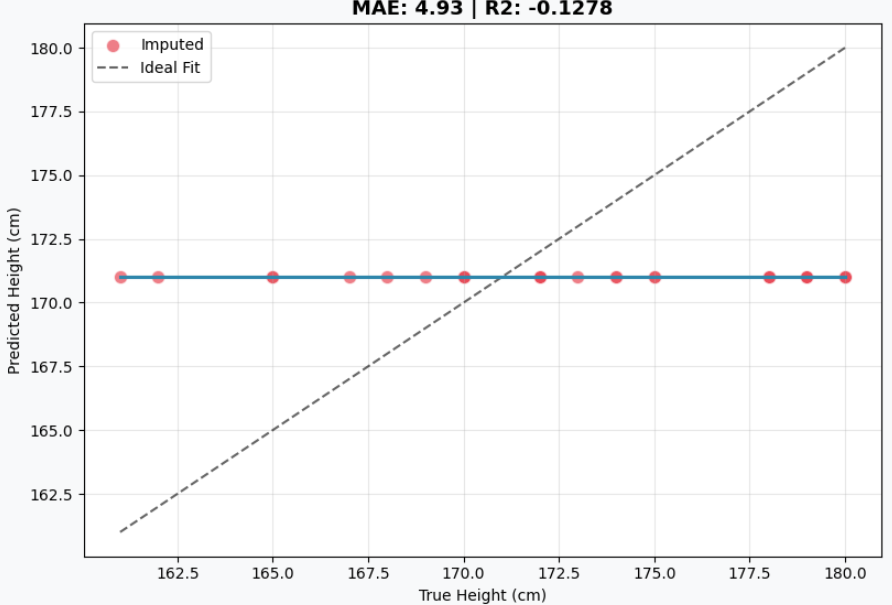
\includegraphics[width=0.8\linewidth]{median_plot.png}
    \caption{Median Imputation (Baseline).}
    \label{fig:plot_median}
\end{figure}

Regarding traditional machine learning, Figure~\ref{fig:plot_mice} and Figure~\ref{fig:plot_mf} show a clearer correlation. While MICE displays a general diagonal trend, it still exhibits significant dispersion, with many points far from the $y=x$ line . In contrast, MissForest provides the most accurate results, with points clustered tightly along the diagonal, confirming its superior performance in capturing feature relationships even with limited data.

% 2. MICE
\begin{figure}[ht]
    \centering
    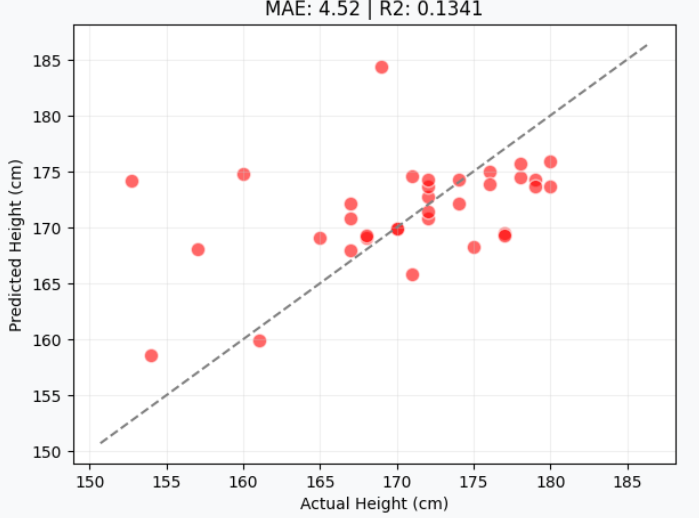
\includegraphics[width=0.8\linewidth]{mice_plot.png}
    \caption{MICE Imputation.}
    \label{fig:plot_mice}
\end{figure}

% 3. MissForest
\begin{figure}[H]
    \centering
    % 同樣設定固定高度，讓它能塞在 MICE 下方
    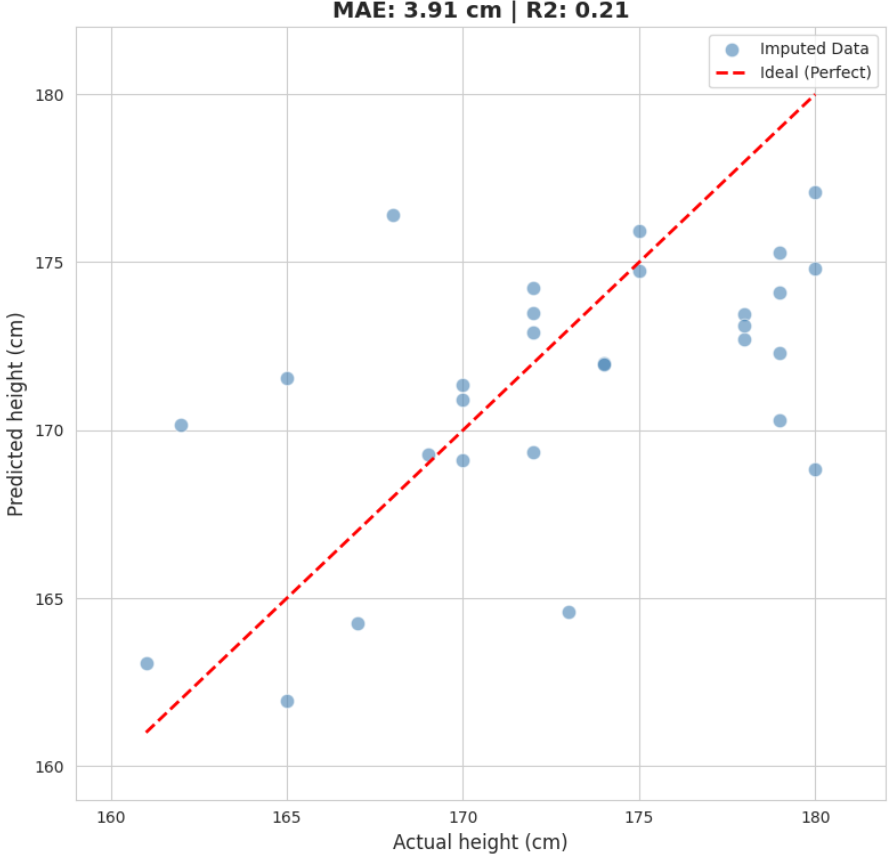
\includegraphics[width=0.8\linewidth, height=4.5cm, keepaspectratio=false]{missforest_plot.png}
    \caption{MissForest Imputation.}
    \label{fig:plot_mf}
\end{figure}

However, the deep learning models fail to produce meaningful predictions in this small-sample scenario. As seen in Figure~\ref{fig:plot_gain} and Figure~\ref{fig:plot_vae}, both GAIN and VAE produce predictions that are highly concentrated around the median value. Instead of aligning with the diagonal $y=x$ line, the imputed points are scattered only around a horizontal band. This indicates that the models have failed to capture any individual variance and are simply outputting values near the statistical average to minimize training loss, which visually explains their poor convergence and negative $R^2$ results.

% 4. GAIN
\begin{figure}[ht]
    \centering
    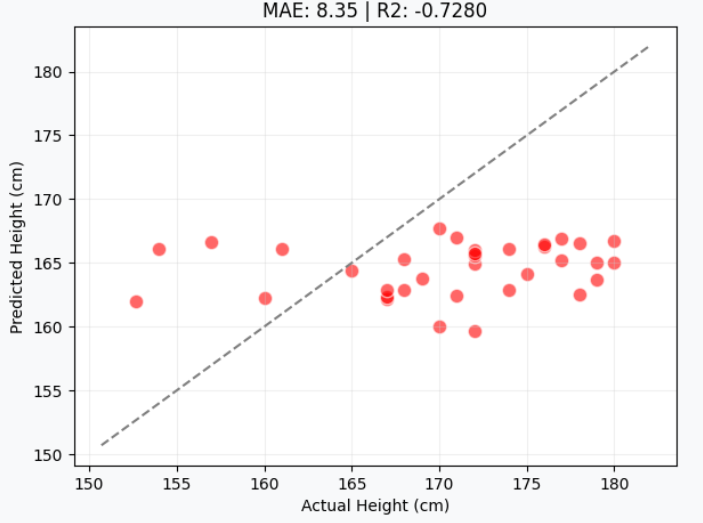
\includegraphics[width=0.8\linewidth]{gain_plot.png}
    \caption{GAIN.}
    \label{fig:plot_gain}
\end{figure}

% 5. VAE
\begin{figure}[ht]
    \centering
    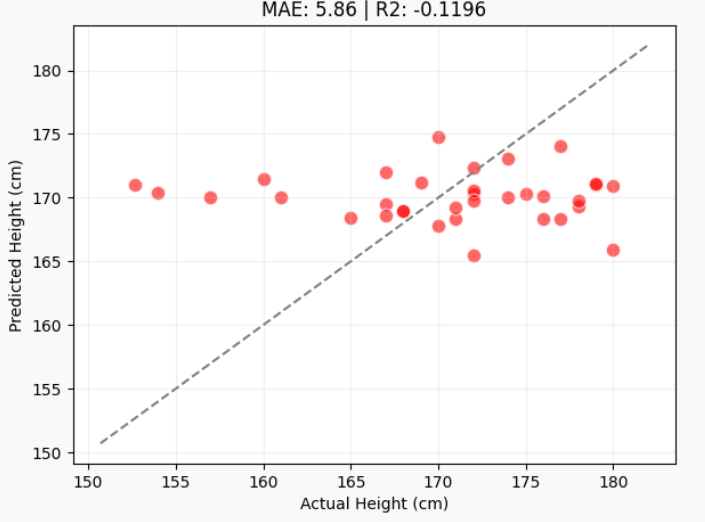
\includegraphics[width=0.8\linewidth]{vae_plot.png}
    \caption{VAE.}
    \label{fig:plot_vae}
\end{figure}

\FloatBarrier

In summary, for small-scale datasets with simple feature dimensions, deep learning models are not the optimal choice for missing value imputation. Their recovery performance often lags behind basic statistical baselines, whereas traditional machine learning like MissForest demonstrates superior robustness. These findings suggest that model selection must prioritize the impact of data scale on algorithmic convergence; pursuing complex models without sufficient data leads to lower imputation fidelity.
\subsubsection{Recovery Performance on Big Dataset}

In the tests using the large-scale dataset (CDC BRFSS), the experimental results show a completely different trend compared to the small-sample tests. When the amount of data increases significantly, the advantages of deep learning models start to appear. According to the data in Table~\ref{tab:cdc_results}, VAE showed a dominant advantage in all evaluation metrics. Its $R^2$ reached the highest in the entire group at 0.9386, and the MAE was only 0.724. This shows that in a big data environment, VAE can accurately learn the data distribution and the complex relationships between features.

In contrast, traditional machine learning methods like MICE and MissForest still maintain good stability, with $R^2$ values of 0.5572 and 0.5664, respectively. However, their recovery accuracy is clearly behind VAE. This proves that while traditional methods can still provide reliable results when dealing with massive amounts of data, their ability to represent data has reached a bottleneck. They find it hard to improve the imputation quality further through big data, unlike certain deep learning models.

It is worth noting that another deep learning model, GAIN, still performs poorly at this stage. The failure of GAIN is mainly due to the gap between distribution matching and point-wise accuracy. While GAIN focuses on making the overall statistical distribution look real to fool the discriminator, it often ignores the exact precision for each individual data point, leading to a low $R^2$. 

Furthermore, GAIN often suffers from ``mode collapse,'' where the generator simply predicts the average height to stay ``safe,'' which explains the horizontal patterns seen in its scatter plots. Another possible reason for this failure is the choice of data encoding. In this experiment, we used Label Encoding , but GAIN is generally more suitable for One-Hot Encoding to handle categorical features correctly. Additionally, the adversarial training process is highly unstable for tabular data, making it difficult to converge even with large datasets. In summary, the large-scale experiment confirms that when the data scale is large enough, deep learning—especially generative models like VAE—has great potential to surpass traditional methods, provided the training is stable.

\begin{table}[h]
\renewcommand{\arraystretch}{1.5}
\centering
\caption{Recovery Performance Comparison - Big Dataset}
\label{tab:cdc_results}
\resizebox{\columnwidth}{!}{ % <--- 開始縮放
    \begin{tabular}{lcccc}
    \toprule
    Method & MAE (cm) & RMSE (cm) & $R^2$ & Bias (cm) \\
    \midrule
    Median Impute & 8.8916 & 10.8688 & -0.0927 & -1.9041 \\
    MICE & 5.4667 & 7.0170 & 0.5572 & 0.0222 \\
    MissForest & 5.4062 & 6.9443 & 0.5664 & 0.0045 \\
    GAIN & 8.118 & 10.0684 & 0.0791 & -2.47 \\
    VAE & 0.724 & 2.576 & 0.9386 & 0.0664 \\
    \bottomrule
    \end{tabular}
} % <--- 結束縮放
\end{table}

In the large-scale dataset (CDC BRFSS) tests, the visual distribution plots reveal significant differences in how algorithms scale with data.

Regarding traditional machine learning, MICE and MissForest (Figure~\ref{fig:cdc_plot_mice} and Figure~\ref{fig:cdc_plot_mf}) show improved stability compared to small samples. The points begin to align more clearly with the diagonal line, proving that the models successfully learned the linear trends between features. However, their density along the diagonal is lower than VAE, suggesting that traditional ensemble methods reach a performance bottleneck when dealing with massive datasets.

% 第 1 張：Median 獨立出來
\begin{figure}[htbp]
    \centering
    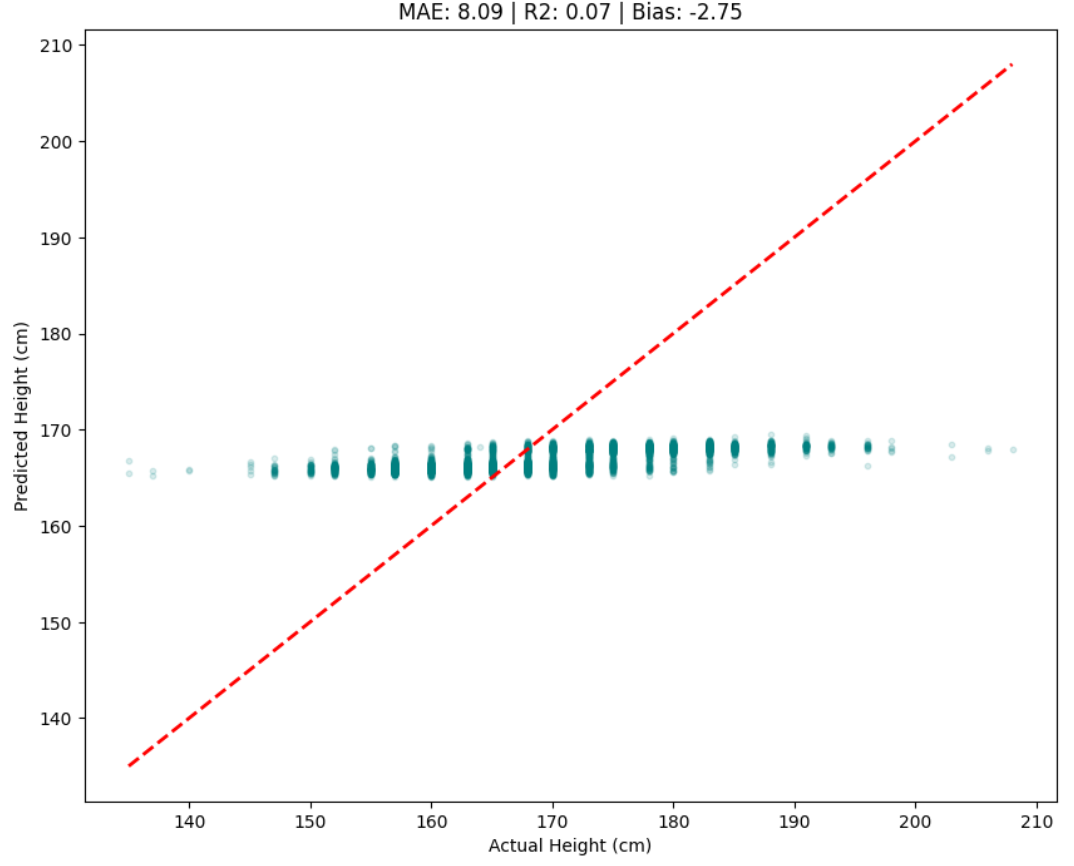
\includegraphics[width=0.85\linewidth]{median-bigdata.png}
    \caption{Median Imputation. Similar to the small dataset, it fails to capture any individual variance.}
    \label{fig:cdc_plot_median}
\end{figure}

% 第 2 張：MICE 獨立出來
\begin{figure}[htbp]
    \centering
    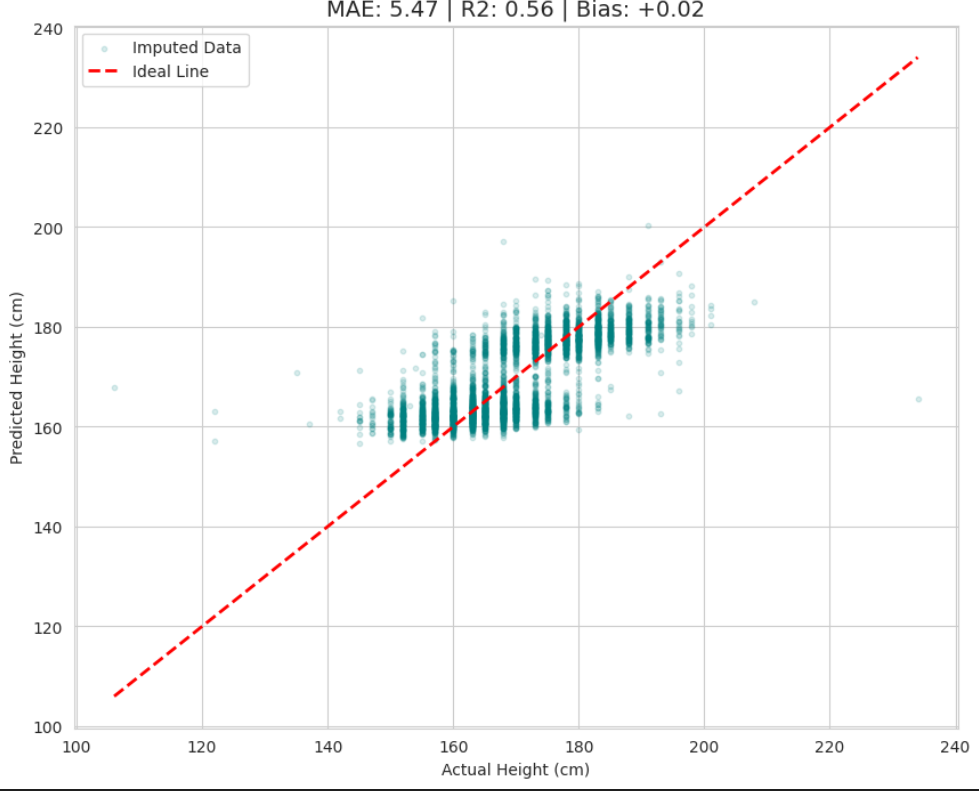
\includegraphics[width=0.85\linewidth]{mice_bigdata.png}
    \caption{MICE Imputation. The distribution begins to align with the diagonal, but still shows noticeable spread.}
    \label{fig:cdc_plot_mice}
\end{figure}

% 第 3 張：MissForest 獨立出來
\begin{figure}[htbp]
    \centering
    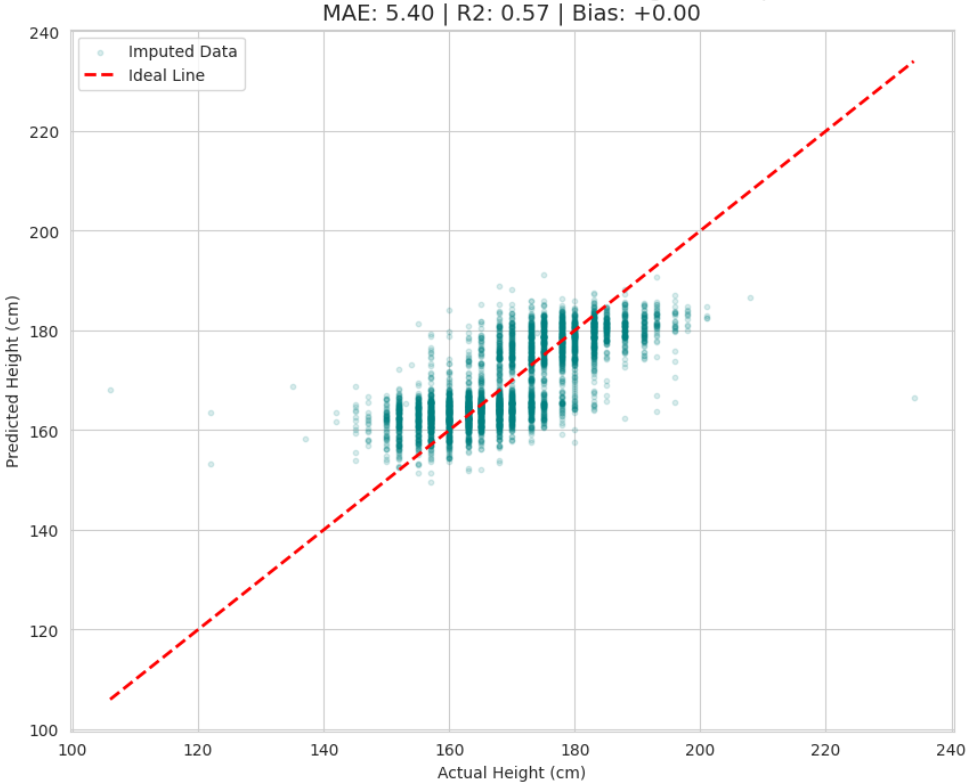
\includegraphics[width=0.85\linewidth]{missforest_bigdata.png}
    \caption{MissForest Imputation. Performance is stable, but the density around the diagonal is lower than VAE.}
    \label{fig:cdc_plot_mf}
\end{figure}


% 4. GAIN (CDC)
\begin{figure}[htbp] % <--- 統一改成 htbp
    \centering
    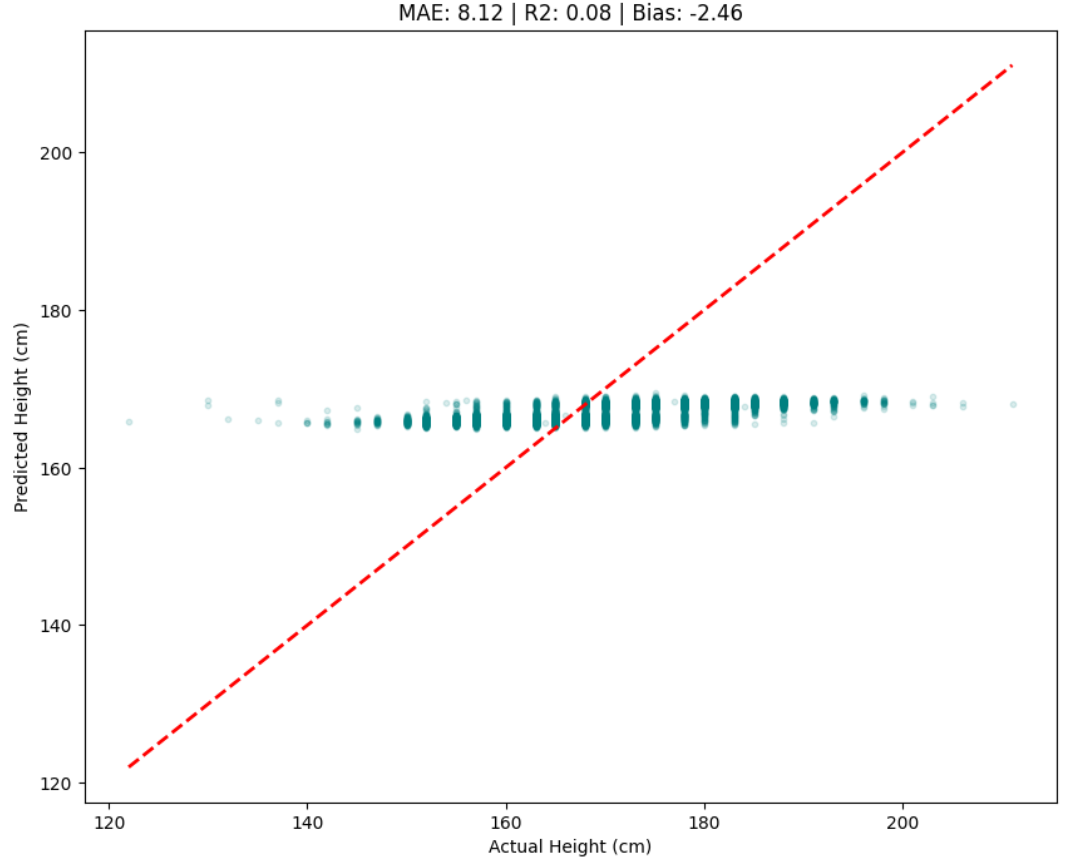
\includegraphics[width=0.75\linewidth]{gain_bigdata.png}
    \caption{GAIN. The points are widely scattered in a horizontal pattern, showing mode collapse around the median.}
    \label{fig:cdc_plot_gain}
\end{figure}

On the other hand, the deep learning models show extreme differences. As seen in Figure~\ref{fig:cdc_plot_gain}, GAIN continues to struggle with convergence. The imputed points are scattered only within a horizontal band around the median, failing to follow the diagonal line. This confirms "mode collapse," where the generator only predicts average values to stay "safe" from the discriminator. In sharp contrast, VAE (Figure~\ref{fig:cdc_plot_vae}) demonstrates superior distribution learning, with points tightly concentrated along the $y=x$ diagonal. With sufficient data support, the latent space of VAE effectively reconstructs the complex underlying logic of tabular data, achieving the highest imputation fidelity in the entire group.


% 5. VAE (CDC)
\begin{figure}[htbp] % <--- 統一改成 htbp
    \centering
    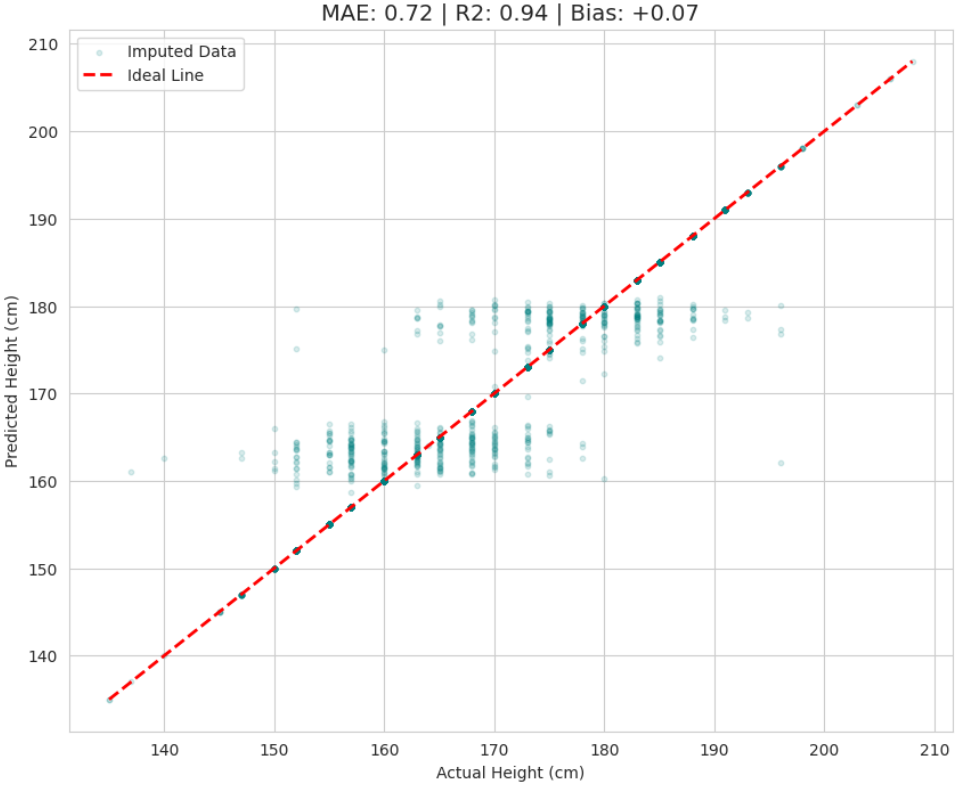
\includegraphics[width=0.75\linewidth]{VAE-bigdata.png}
    \caption{VAE. The points are highly concentrated along the $y=x$ line, visually confirming the $R^2 = 0.9386$ result.}
    \label{fig:cdc_plot_vae}
\end{figure}

% \FloatBarrier % 繼續保持註解掉，讓版面自由流動

In our large-scale experiment, we observed a clear reversal in performance. As the data size grows, the recovery accuracy of traditional machine learning remains stable, but it seems to have a limit. On the other hand, with enough data support, certain deep learning methods show a strong ability to learn features, which greatly improves the imputation accuracy. This proves that for handling missing values in large datasets, generative deep learning models are a better and more promising solution.

\subsection{Phase 2: Downstream Performance Evaluation}
\subsubsection{Experimental Objectives and Model Selection}

The main goal of this phase is to verify the relationship between imputation quality and actual application effects. In Phase 1, we evaluated the data recovery accuracy. However, the method with the highest accuracy does not always mean it provides the most useful feature information for future tasks. Therefore, Phase 2 focuses on evaluating the effects of different imputation strategies on the gender classification task.

We chose the "Boy or Girl" dataset as our research object. This dataset includes various numerical and categorical features, which can effectively simulate complex tabular data environments. The dataset itself already contains a large amount of original missing values, and its distribution fits the Missing at Random (MAR) mechanism. We used these natural missing values directly for the experiments to reflect the logic of correlated missing data in real-world scenarios.

\subsubsection{Experimental Design and Evaluation Metrics}

To explore how imputation algorithms affect different types of data (numerical and categorical), we divided the imputation process into three main scenarios for comparison:

\begin{itemize}
    \item \textbf{Numerical Imputation (Model) + Categorical Imputation (Unknown):} We only use specific algorithms to fill numerical features like height, weight, and IQ. Categorical features like star sign or phone OS are filled with "Unknown." This design helps us observe how the quality of numerical data recovery alone contributes to the classification task.
    \item \textbf{Baseline (Median/Mode) + Model Imputation:} Numerical features are filled with the median, while categorical features are filled using the target algorithm. This scenario is used to test if the algorithm performs better than simple statistical baselines when handling discrete categorical data.
    \item \textbf{Full Imputation:} Both numerical and categorical features are processed by the same algorithm (such as MissForest or VAE). This evaluates the overall performance of the imputation plan in capturing complex relationships within "mixed data."
\end{itemize}
In all scenarios, the downstream gender prediction model uses the \textbf{LightGBM} classifier. To ensure fairness and reproducibility, the core hyperparameters of the classifier (such as learning rate and number of leaves) remain unchanged. The only variable in the experiment is the imputation method used for the input data.

Since the dataset has a clear class imbalance (the proportion of Gender 1 is much higher than Gender 2), Accuracy alone is not enough to show model performance. Therefore, we use the following metrics for a comprehensive evaluation. The evaluation metrics are defined as follows.

Accuracy measures the overall proportion of correct predictions:
\begin{equation}
Accuracy = \frac{TP + TN}{TP + TN + FP + FN}
\end{equation}
Precision and Recall are used to measure the accuracy of positive predictions and the ability to find all positive cases, respectively:
\begin{equation}
Precision = \frac{TP}{TP + FP}, \quad Recall = \frac{TP}{TP + FN}
\end{equation}
The F1-Score, which is the harmonic mean of Precision and Recall, serves as our core metric for handling class imbalance:
\begin{equation}
F1\text{-}Score = 2 \times \frac{Precision \times Recall}{Precision + Recall}
\end{equation}
Additionally, we use ROC-AUC to check the model's ability to distinguish between classes at various thresholds, and the Confusion Matrix to visualize where the model mistakes one gender for another. This comprehensive analysis helps determine if the imputed data successfully preserves the key physical differences between genders.

\subsubsection{Results and Discussion}

Based on the experimental data in Table~\ref{tab:phase2_results}, we analyzed how different imputation methods affect the gender classification task on the \textit{Boy or Girl} dataset. The results show that traditional machine learning methods, specifically MICE and MissForest, generally perform better than the Control Group and deep learning models. Among all configurations, MissForest using numerical imputation with "Unknown" categorical data achieved the highest Accuracy 0.8913 and F1-Score 0.7723. This proves that for small tabular datasets, MissForest can effectively recover key physical features like height and weight, which significantly improves the prediction performance of the LightGBM classifier.

For both MICE and MissForest, filling only numerical features while leaving categorical data as "Unknown" performed slightly better than Full Imputation. For example, the Accuracy of MissForest dropped from 0.8913 to 0.8842 when categorical features were also imputed. This suggests that in small-sample scenarios, imputing highly uncertain categorical features might introduce noise that slightly reduces classification precision. However, the Full Imputation version of MissForest reached the highest Recall 0.7383, meaning it was the best at finding the minority class.

On the other hand, the performance of deep learning models was relatively average. GAIN with full imputation only achieved an Accuracy of 0.8747 and an F1-Score of 0.7104, which is identical to the Control Group. This indicates that the data generated by GAIN did not provide extra useful information for classification. VAE performed slightly better than GAIN, reaching an F1-Score of 0.7435 with full imputation, but it still behind MICE and MissForest. These results confirm the core finding of this study, when dealing with small mixed tabular data, generative models like GAIN and VAE are limited by the sample size, making their data utility lower than traditional ensemble methods like MissForest.
\begin{table}[ht]
\centering
\caption{Downstream Classification Performance on \textit{Boy or Girl} Dataset}
\label{tab:phase2_results}
\renewcommand{\arraystretch}{1.5} % 增加行間距，讓表格不擁擠
\setlength{\tabcolsep}{5pt}      % 調整欄間距
\resizebox{\columnwidth}{!}{
\begin{tabular}{lccccccc}
\toprule
Method & Numerical & Categorical & Acc & Precision & Recall & F1-Score & ROC-AUC \\
\midrule
Control Group & Median & ``Unknown'' & 0.8747 & 0.8553 & 0.6075 & 0.7104 & 0.9089 \\
MICE & MICE & ``Unknown'' & 0.8913 & 0.8280 & 0.7196 & 0.7700 & 0.8980 \\
MissForest & MissForest & ``Unknown'' & 0.8913 & 0.8211 & 0.7290 & 0.7723 & 0.8979 \\
MissForest & MissForest & MissForest & 0.8842 & 0.7900 & 0.7383 & 0.7633 & 0.8865 \\
GAIN & GAIN & ``Unknown'' & 0.8771 & 0.8161 & 0.6636 & 0.7320 & 0.9035 \\
GAIN & Median & GAIN & 0.8723 & 0.8354 & 0.6168 & 0.7097 & 0.9113 \\
GAIN & GAIN & GAIN & 0.8747 & 0.8553 & 0.6075 & 0.7104 & 0.9035 \\
VAE & VAE & ``Unknown'' & 0.8794 & 0.8784 & 0.6075 & 0.7128 & 0.9035 \\
VAE & Median & VAE & 0.8652 & 0.8678 & 0.5514 & 0.6743 & 0.9149 \\
VAE & VAE & VAE & 0.8842 & 0.8452 & 0.6636 & 0.7435 & 0.8850 \\
\bottomrule
\end{tabular}
}
\vspace{2pt}
\begin{flushleft}
\footnotesize{Note: ``Unknown'' indicates that categorical features were not imputed but replaced with a constant label to evaluate the specific impact of numerical feature recovery.}
\end{flushleft}
\end{table}

\subsubsection{Visual Analysis and Discussion}

The analysis of the Confusion Matrices reveals the model's ability to identify gender groups, especially the minority class (Gender 2). As shown in Figure~\ref{fig:cm_control}, the Control Group misclassifies 42 females as males, indicating limited sensitivity to the minority class. In contrast, Figure~\ref{fig:cm_missforest} shows that MissForest (Numerical + Unknown) achieves the best results, with the clearest diagonal distribution and only 29 misclassifications. This proves that this strategy preserves the most discriminative features. Finally, as seen in Figure~\ref{fig:cm_vae}, VAE performs better than the baseline but still has 36 misclassifications, likely due to noise introduced during imputation.

% --- 混淆矩陣圖片開始 ---
\begin{figure}[ht]
    \centering
    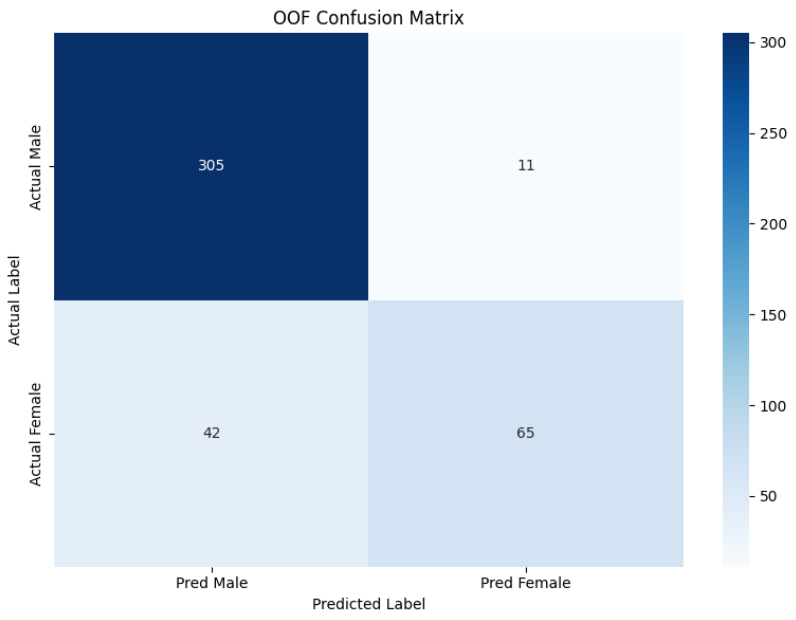
\includegraphics[width=0.75\linewidth]{confusion_control.png}
    \caption{Confusion Matrix: Control Group. The model shows lower sensitivity to the minority class.}
    \label{fig:cm_control}
\end{figure}

\begin{figure}[ht]
    \centering
    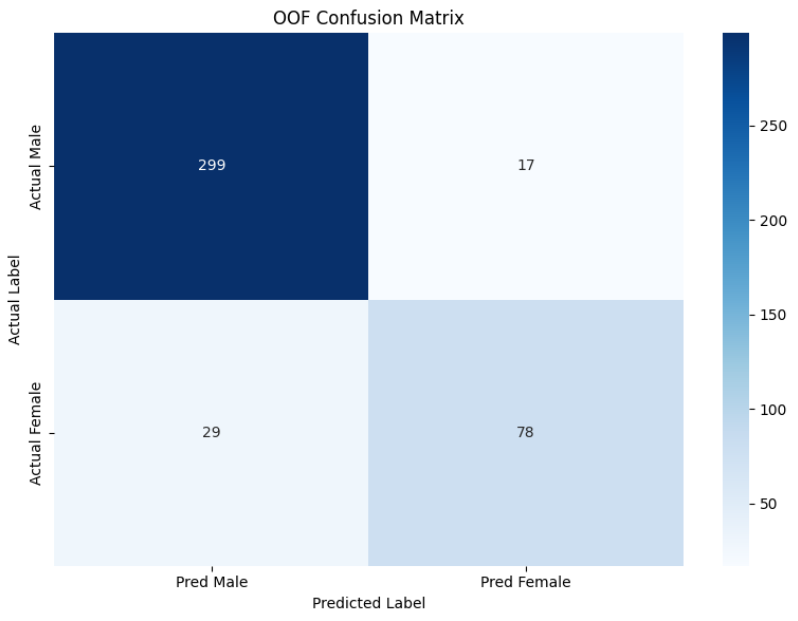
\includegraphics[width=0.75\linewidth]{confusion_missforest_num.png}
    \caption{Confusion Matrix: MissForest (Numerical + Unknown). This shows the clearest diagonal and best F1-Score.}
    \label{fig:cm_missforest}
\end{figure}

\begin{figure}[ht]
    \centering
    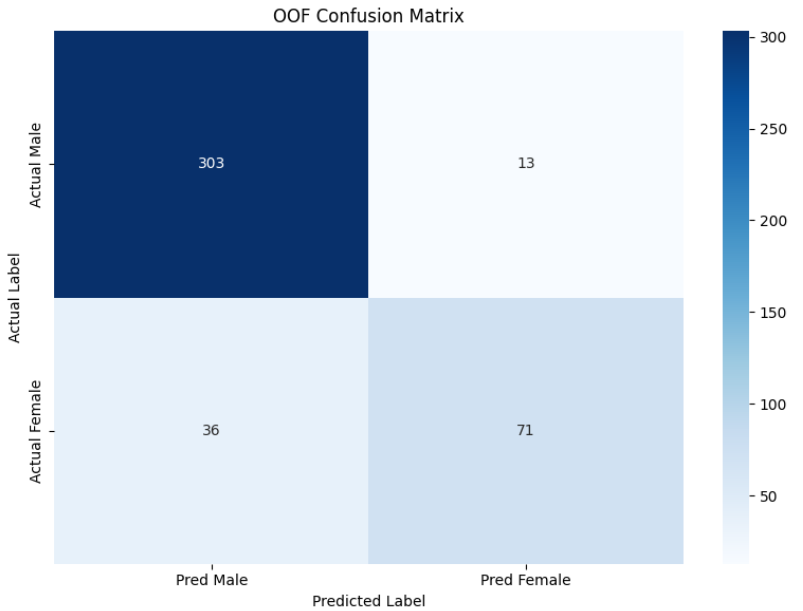
\includegraphics[width=0.75\linewidth]{confusion_vae_full.png}
    \caption{Confusion Matrix: VAE (Full Imputation). Increased noise leads to more misclassifications than MissForest.}
    \label{fig:cm_vae}
\end{figure}
% --- 混淆矩陣圖片結束 ---

% \FloatBarrier % <--- 1. 把它註解掉，不要強制阻擋排版流動

Next, we use ROC Curves to check the stability of the LightGBM classifier. As shown in Figure~\ref{fig:roc_control}, Figure~\ref{fig:roc_missforest}, and Figure~\ref{fig:roc_vae}, all three cases achieve an AUC above 0.88, representing excellent predictive performance. Although the Control Group has the highest AUC (0.909), this is mainly due to its consistent predictions on the majority class. MissForest and VAE maintain strong discriminative power while providing richer feature information, ensuring stability in real-world applications.

% --- 獨立把 14 號圖抽出來，它就會自動塞進左欄文字下方 ---
\begin{figure}[htbp] 
    \centering
    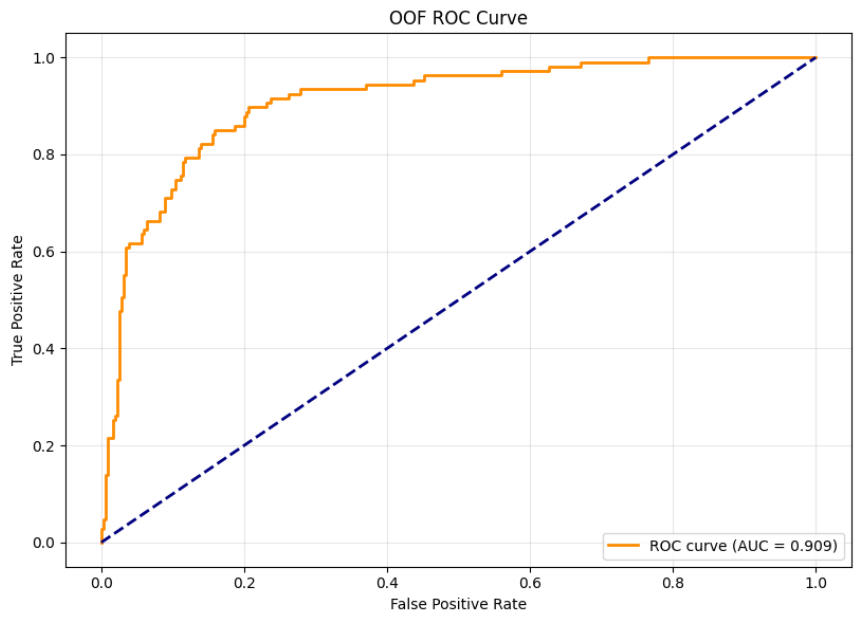
\includegraphics[width=0.75\linewidth]{roc_control.png}
    \caption{ROC Curve: Control Group. High AUC reflects stability on original distributions.}
    \label{fig:roc_control}
\end{figure}

% --- 15、16 號圖綁在一起，LaTeX 會自動把這包推去右欄頂部 ---
\begin{figure}[htbp]
    \centering
    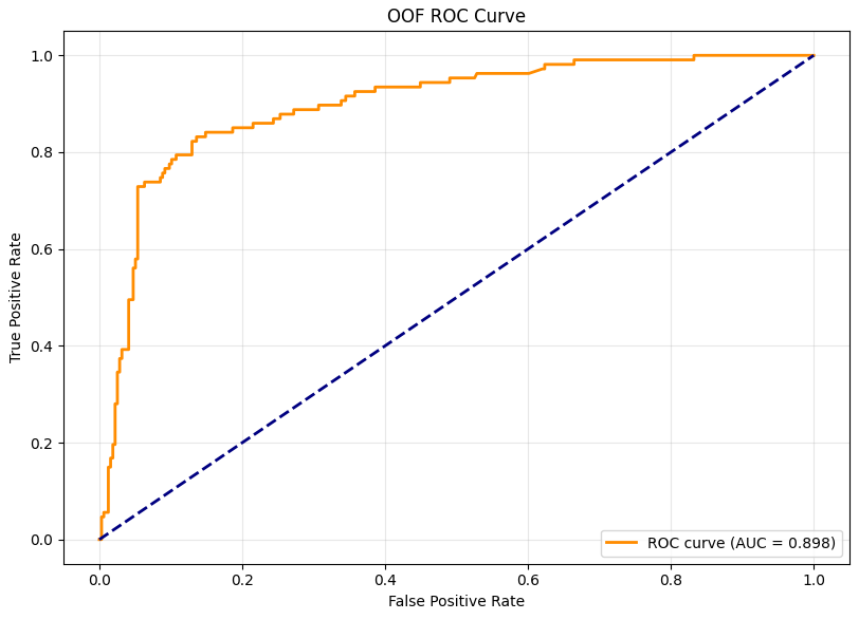
\includegraphics[width=0.75\linewidth]{roc_missforest_num.png}
    \caption{ROC Curve: MissForest (Numerical + Unknown). The model maintains robust discriminative power.}
    \label{fig:roc_missforest}
    
    \vspace{1.5em} % 15、16 號之間的垂直距離
    
    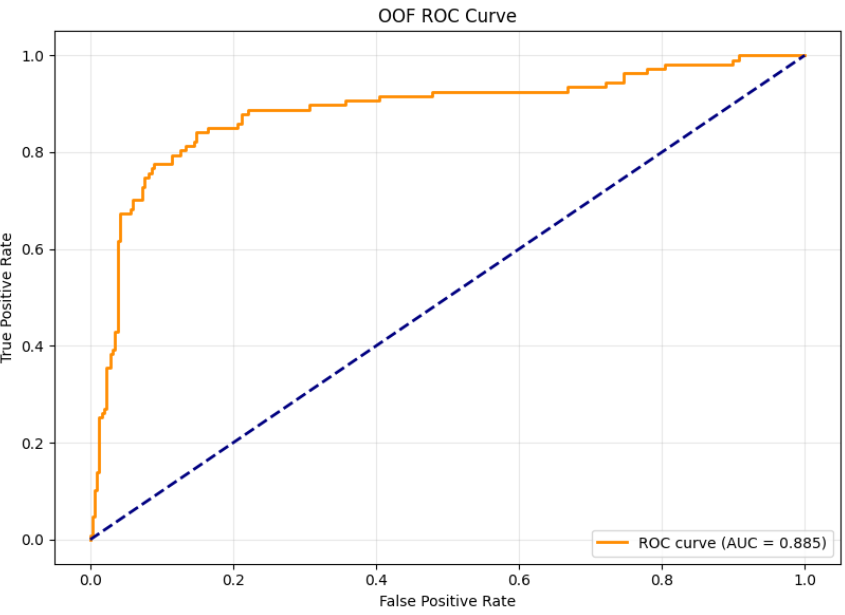
\includegraphics[width=0.75\linewidth]{roc_vae_full.png}
    \caption{ROC Curve: VAE (Full Imputation). Shows a slight decrease in power due to noise on a small sample size.}
    \label{fig:roc_vae}
\end{figure}
% --- ROC 曲線圖片結束 ---

% 築起隱形牆，確保結論一定在所有圖片之後
\FloatBarrier

\section{Conclusion}

This research confirms that there is no single "best" algorithm for tabular data imputation. Its performance depends heavily on the data scale and the missing mechanisms, such as MCAR, MAR, or MNAR. 

Our analysis and experimental results show that in small-sample environments (such as the \textit{Boy or Girl} dataset), traditional models like MissForest perform better. Because of their strong inductive bias, they capture non-linear relationships more accurately and offer higher stability and F1-Scores than deep learning models like GAIN and VAE. However, as the data size grows to a large scale (such as the \textit{CDC BRFSS} dataset), deep learning models like VAE show superior performance. By learning latent space distributions, VAE can accurately reconstruct the underlying data logic and surpass the limits of traditional machine learning. 

In summary, practitioners should first understand the characteristics of their dataset—including the missingness type, data size, and time cost—to achieve the best results in model training.


\section{References} 
\printbibliography[heading=none] % 加上 [heading=none] 強制關閉它內建的標題

\section{Work Division}
The authors confirm and agree that their work description and contribution are correct.

\begin{table}[h]
    \centering
    % 加入 | 來畫出垂直線，稍微縮小一點比例避免加上框線後超出邊界
    \begin{tabular}{| p{0.22\linewidth} | p{0.48\linewidth} | c |}
        \hline % 頂部水平線
        \textbf{Name} & \textbf{Work description} & \textbf{Contribution} \\
        \hline % 標題下方的水平線
        
        \raggedright Ai-Ting, Lin \newline 113427013 & 
        \raggedright 1. Literature search \newline 
        2. Reviewing traditional Machine Learning imputation methods \newline 
        3. Drafting Sections 2, 3 & 
        25\% \\
        \hline % 第一位作者下方的水平線
        
        \raggedright Li-Feng, Chen \newline 114423006 & 
        \raggedright 1. Literature search \newline 
        2. Empirical experiments design and evaluation \newline 
        3. Drafting Section 4 & 
        25\% \\
        \hline % 第二位作者下方的水平線
        
        \raggedright Jia-Hua, Peng \newline 114423056 & 
        \raggedright 1. Literature search \newline 
        2. Overall manuscript synthesis and formatting \newline 
        3. Drafting Sections 1, 5, Abstract & 
        25\% \\
        \hline % 第三位作者下方的水平線
        
        \raggedright Xin-Ping, Wu \newline 114423067 & 
        \raggedright 1. Literature search \newline 
        2. Reviewing Deep Learning imputation methods \newline 
        3. Drafting Sections 2,3 & 
        25\% \\
        \hline % 底部水平線
        
    \end{tabular}
\end{table}


\end{document}